\section{はじめに}
現在我々は多くの情報の中で生活している。
SNSやニュースなどはインターネット上に流れていて簡単に見ることができるが、
誰が今何を考えているのか、どこにいて何をしているのかといった情報も知りたいことがある。
それを実現するためにはありとあらゆる情報を簡単にアウトプットできて、それらを見ることが
できるシステムが必要である。

現在ある、情報を見るためのインタフェースの工夫として、
\begin{itemize}
\item タイムライン表示
\item インフォメーションダッシュボード
\item スタンプ
\end{itemize}
の3つを紹介する。

タイムライン表示は「Twitter」「Facebook」「LINE」等において、
図\ref{twitter}のように投稿を時系列に並べて表示したものだ。
タイムライン表示は情報を後から時間を遡って見るには便利だが、
投稿数の多い人ばかりが目立ってしまったり、リアルタイムに何かを知りたい時に
同時に多数の投稿があると流れて見えなくなってしまったりすることがある。

インフォメーションダッシュボード(図\ref{azure})は、
単一の画面に複数のリアルタイム情報をタイル状に並べて表示するものだ。
インフォメーションダッシュボードはセンサの値や株価など常に値が変化していくものをたくさん並べて、
ひと目で把握するのに非常に便利なインタフェースである。
しかし、表示領域が限られているため、長いテキストを表示するには適していない。

スタンプは大型のピクトグラムを用いたコミュニケーションだ。
スタンプはテキストで記述するのが難しい表現や感情を伝えたり、
テキストを考えて入力するよりも速くて簡単であったりすることから、
近年LINEやFacebookメッセンジャー、オンラインゲームなどで広く利用されている。

そこで、このスタンプをダッシュボードのセルに表示することで、
ダッシュボードとスタンプベースのコミュニケーションを組み合わせた視覚化システム
『わかるらんど』を開発した。
『わかるらんど』は単純なアーキテクチャで、人の感情や現在の状況、
IoT機器の情報などをリアルタイムに視覚化するシステムで、
非常に汎用なダッシュボードとして利用することができる。

\begin{figure}[h]
\centering
\fbox{
  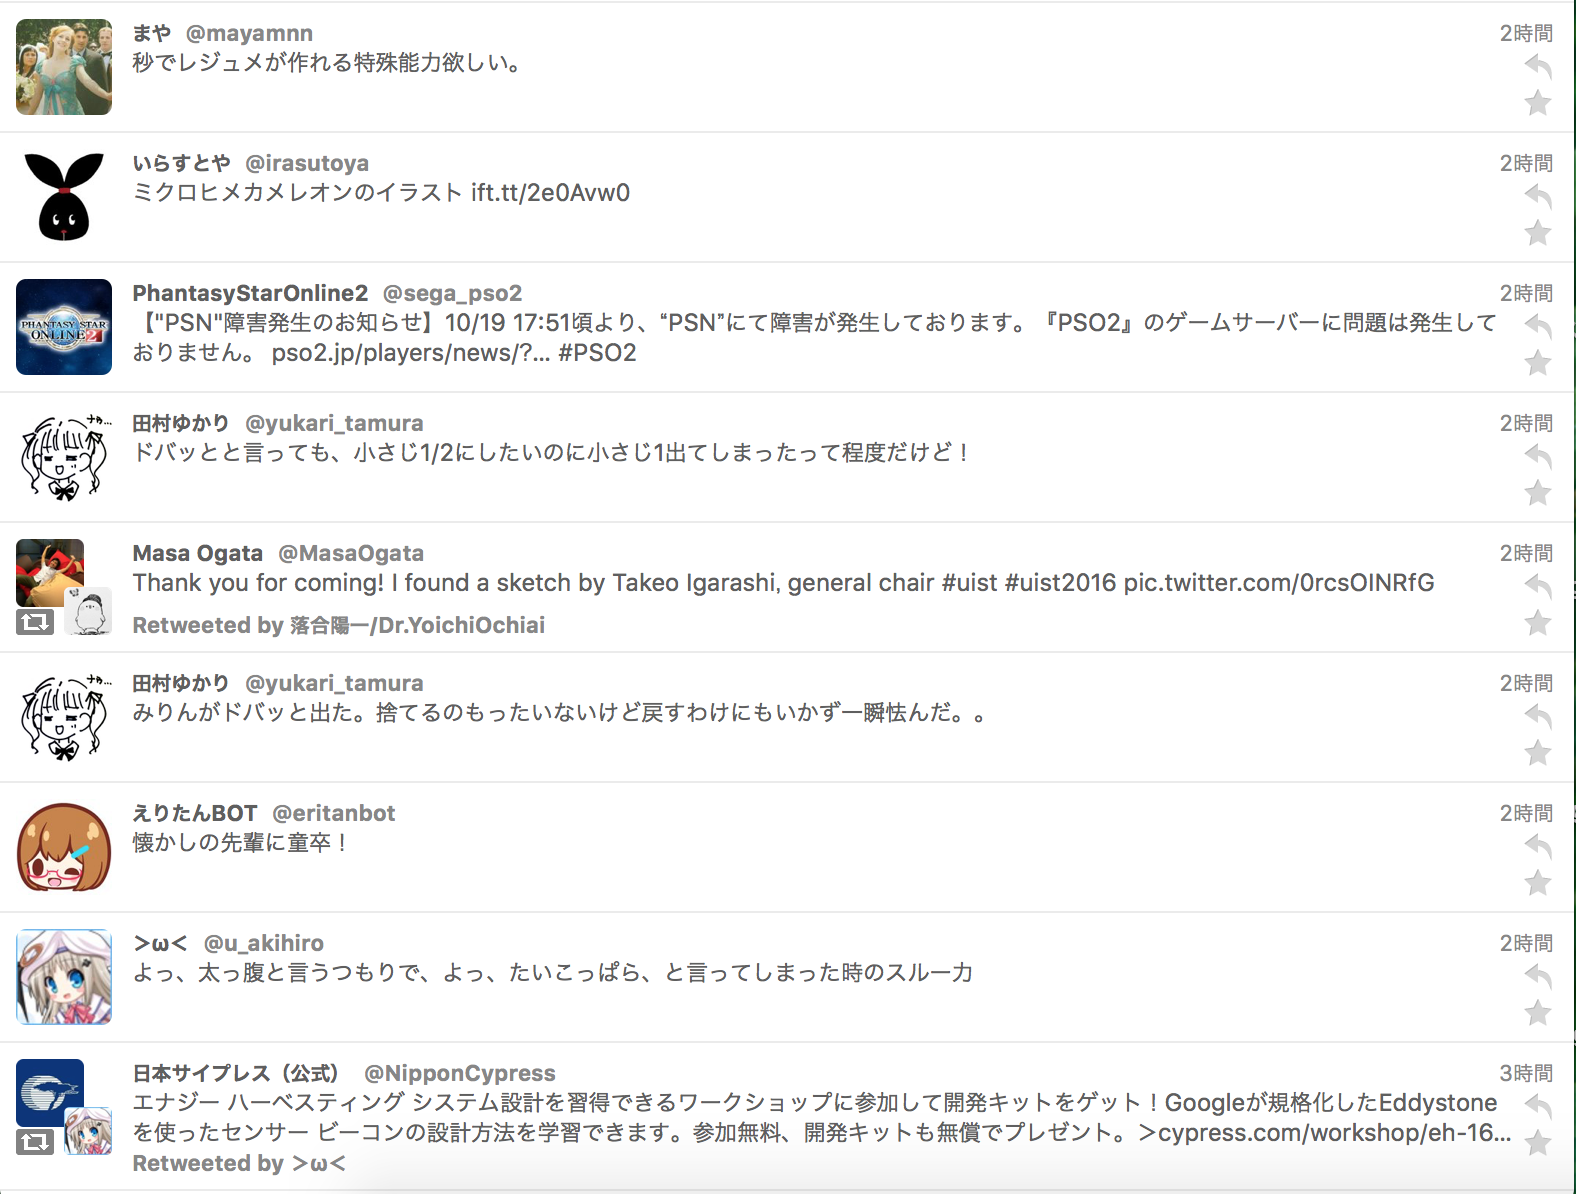
\includegraphics[width=7cm]{images/twitter.png}
}
\caption{Twitterのタイムライン}
\label{twitter}
\end{figure}


\begin{figure}[h]
\centering
\fbox{
  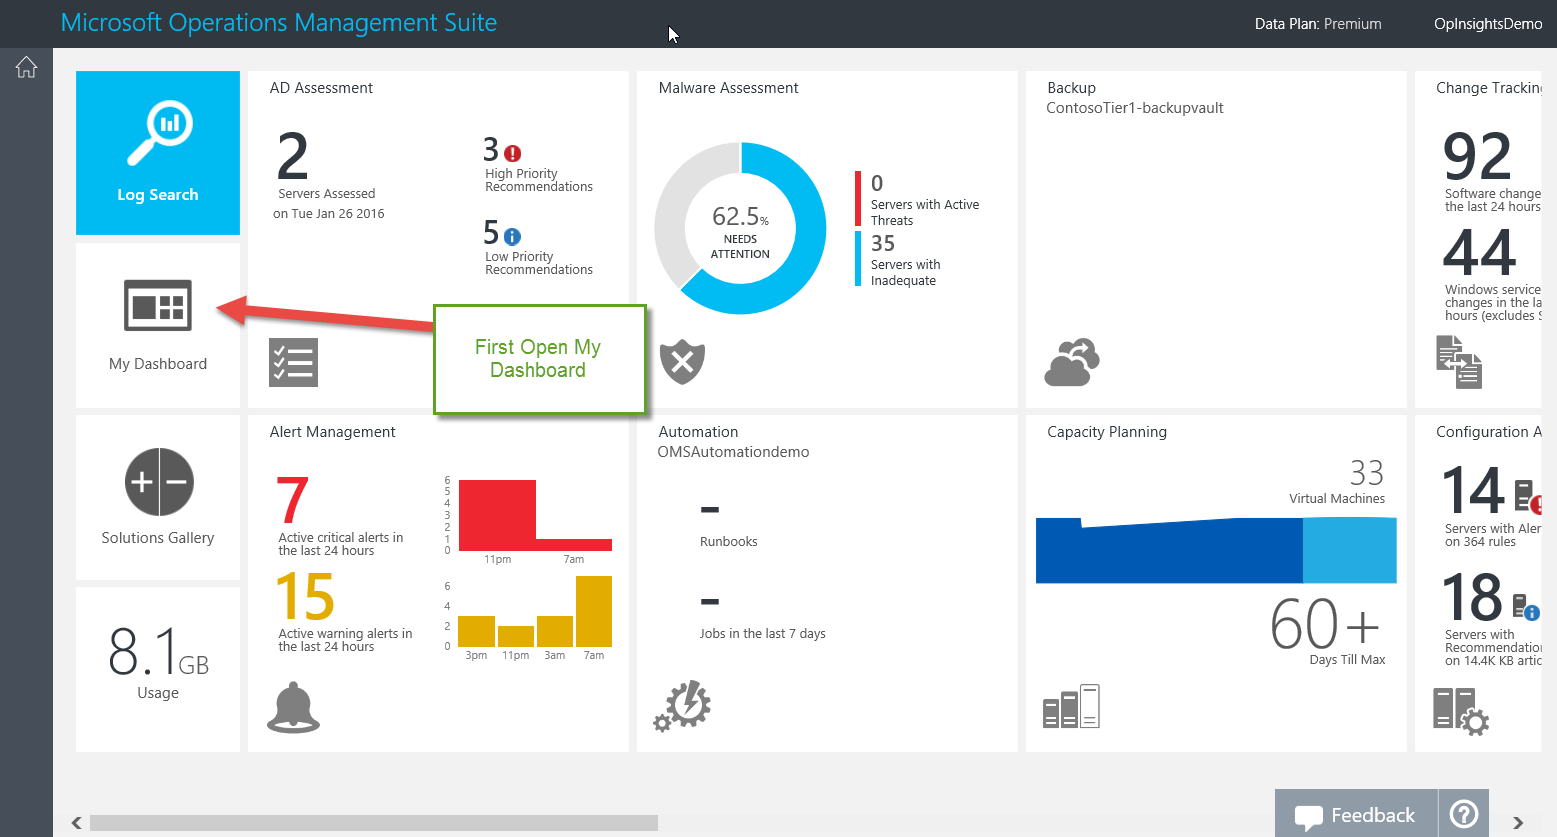
\includegraphics[width=7cm]{images/azure.png}
}
\caption{Microsoft Azureのダッシュボード}
\label{asure}
\end{figure}